\documentclass[12pt]{article}
\usepackage[utf8]{inputenc}
%\usepackage[margin=1in]{geometry}
\usepackage{amssymb}
\usepackage{amsmath}
\usepackage{mathtools}
\usepackage{amsthm}
\usepackage{setspace}
\usepackage{cancel}
\usepackage{bbm}
\usepackage{pgfplots}
\usepackage{listings}

\usetikzlibrary{arrows, calc, patterns, shapes}
  \pgfplotsset{compat=1.15}
\renewcommand{\baselinestretch}{1.25}
\newcommand\sbullet[1][.5]{\mathbin{\vcenter{\hbox{\scalebox{#1}{$\bullet$}}}}}
\newcommand{\indep}{\perp \hspace{-.5 em} \perp}
\def\E{\mathbb{E}}
\def\e{\mathcal{E}}
\def\d{\mathcal{D}}
\def\I{I_n}
\def\l{\ell}
\def\sumn{\sum^n_{i=1}}
\def\i{\mathcal{J}}
\def\x{\mathbf{X}}
\def\inv{^{-1}}
\def\f{Fréchet }
\newcommand{\til}[1]{\underset{\sim}{#1}}
\newcommand\expp[1]{\exp\bigg\{#1\bigg\}}
\newcommand\der[2]{\frac{\partial #1}{\partial #2}}
\newcommand{\ds}{\displaystyle}
\lstset{frame=tb,
  language=Python,
  aboveskip=3mm,
  belowskip=3mm,
  showstringspaces=false,
  columns=flexible,
  basicstyle={\small\ttfamily},
  numbers=none,
  numberstyle=\tiny\color{gray},
  keywordstyle=\color{blue},
  commentstyle=\color{red},
  stringstyle=\color{mauve},
  breaklines=true,
  breakatwhitespace=true,
  tabsize=3
}
\theoremstyle{definition}
\newtheorem{theorem}{Theorem}

\theoremstyle{definition}
\newtheorem{definition}{Definition}

\newtheorem{example}{Example}[section]

\let\inf\infty
\title{Max-Linear Models and Extreme Value Copulas}
\author{Jean-Yves Djamen }
\date{Fall 2019}

\begin{document}

\maketitle
\tableofcontents{}
\pagebreak

\section{Preface}
This paper aims to report on the use of Copula theory as an approach to simplifying max-linear models. Such models arise from a specific instance of probabilistic graphical representations: Bayesian networks. Bayesian networks are in the form Directed Acyclic Graphs (DAG) where the nodes are used to represent random variables and any edge that connects two nodes represents dependence or direct influence (\cite{bayes} chapter 3). In Bayesian graphs, each node is said to be conditionally independent of its non descendants given its immediate parents. This conditional independence is termed the Markov property.

\subsection{Notation}
This report is paired with a document containing code to exhibit practical applications of the theory proposed. The document \textit{ML-Models Code.Rmd} is available as an r markdown document or a pdf and should be attached to this copy of the report.
\subsubsection{Graphs}
\begin{minipage}{0.6 \linewidth}
Consider the graph to the right. Throughout this paper, the following notation will be used:
\begin{itemize}
    \item $an(i)$: Ancestors of node $i$
    \item $An(i)$: $an(i)\cup \{i\}$
    \item $nd(i)$: Non descendants of node $i$
    \item $pa(i)$: immediate parents of node $i$
    \item $Pa(i)$: $pa(i) \cup \{i\}$
    \item $P_{ji}$: all paths from $j$ to $i$
\end{itemize}
\end{minipage}
\begin{minipage}{0.1 \linewidth}
~
\end{minipage}
\begin{minipage}{0.2 \linewidth}
\begin{center}
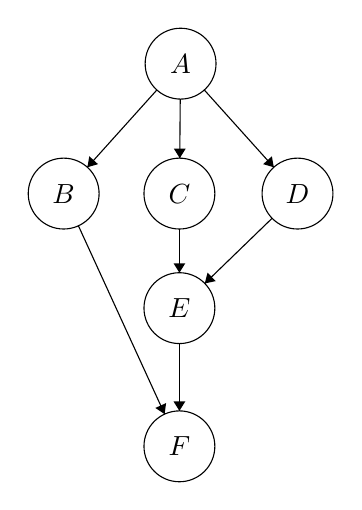
\begin{tikzpicture}[scale=0.15]
\tikzstyle{every node}+=[inner sep=0pt]
\draw [black] (39.9,-6.2) circle (3);
\draw (39.9,-6.2) node {$A$};
\draw [black] (30,-17.2) circle (3);
\draw (30,-17.2) node {$B$};
\draw [black] (39.8,-17.2) circle (3);
\draw (39.8,-17.2) node {$C$};
\draw [black] (49.8,-17.2) circle (3);
\draw (49.8,-17.2) node {$D$};
\draw [black] (39.8,-26.9) circle (3);
\draw (39.8,-26.9) node {$E$};
\draw [black] (39.8,-38.6) circle (3);
\draw (39.8,-38.6) node {$F$};
\draw [black] (37.89,-8.43) -- (32.01,-14.97);
\fill [black] (32.01,-14.97) -- (32.91,-14.71) -- (32.17,-14.04);
\draw [black] (39.87,-9.2) -- (39.83,-14.2);
\fill [black] (39.83,-14.2) -- (40.33,-13.4) -- (39.33,-13.4);
\draw [black] (41.91,-8.43) -- (47.79,-14.97);
\fill [black] (47.79,-14.97) -- (47.63,-14.04) -- (46.89,-14.71);
\draw [black] (47.65,-19.29) -- (41.95,-24.81);
\fill [black] (41.95,-24.81) -- (42.88,-24.61) -- (42.18,-23.9);
\draw [black] (39.8,-20.2) -- (39.8,-23.9);
\fill [black] (39.8,-23.9) -- (40.3,-23.1) -- (39.3,-23.1);
\draw [black] (31.25,-19.93) -- (38.55,-35.87);
\fill [black] (38.55,-35.87) -- (38.67,-34.94) -- (37.76,-35.35);
\draw [black] (39.8,-29.9) -- (39.8,-35.6);
\fill [black] (39.8,-35.6) -- (40.3,-34.8) -- (39.3,-34.8);
\end{tikzpicture}
\end{center}
\end{minipage}
\begin{example}
\begin{align*}
    &pa(A)=\{\varnothing\}&&  pa(C)=\{A\} &&  pa(E)=\{C,D\}\\
    &an(A)=\{\varnothing\}&&an(C)=\{A\}&&an(E)= \{A,C,D\}\\
    &nd(A)=\{\varnothing\}&&nd(C)=\{A,B,D\} &&nd(E)=\{A,B,C,D\}\\
    &P_{BC}=\{\varnothing\}&& P_{AB}=\{AB\} &&P_{AE}=\{ACE,ADE\}
\end{align*}
\end{example}
\subsubsection{Random Variables}
As is convention, a single capital letter will denote a one dimensional random variable whereas a bold capital letter will denote a collection of random variables in a vector.
\begin{example}
Let $\ds X_i \overset{\tiny{iid}}{\thicksim} \mathcal{N}(\mu,\sigma^2)$ for $i=1, \hdots, d$. Then $\mathbf{X}\thicksim \mathcal{N}_d(\vec{\mu}, \Sigma)$ where $\mathbf{X}$ corresponds to:
\begin{align*}
    \mathbf{X}=\begin{bmatrix}X_1\\ X_2 \\ \vdots \\ X_d
    \end{bmatrix}
\end{align*}
\end{example}
\subsubsection{Operators}
The operator $\vee$ is used to symbolise the maximum of two values. When indexing over a set, the operator $\bigvee$ is used.
\begin{example}
Let $A=\{1,4,5,6\}$.
\begin{align*}
    A_1\vee A_2=4 && \bigvee_{a \in A}a=6 
\end{align*}
\end{example}
\pagebreak
\section{Introduction to Max-Linear Model}
\subsection{Recursive Structural Equation Models}
Before we begin our investigation into max-linear models, we must first consider \textbf{recursive structural equation models} (recursive SEM). Below is a definition of a recursive SEM as described in \cite{mlmodels}.
\begin{definition} Given a DAG $\mathcal{D}=(V,E)$ and the following:
\begin{enumerate}
    \item Node set $V=\{1,\hdots, d\}$
    \item Corresponding independent noise variables $\{Z_1,\hdots, Z_d\}$
    \item Edge set $E=\{(k,i):i \in V \ \text{and } k \in pa(i)\}$
    \item A set of real valued measurable functions $\{f_1, \hdots, f_d\}$
\end{enumerate}
A recursive SEM takes the form:
\begin{align*}
    &X_i=f_i(\mathbf{X}_{pa(i)},Z_i) && \forall i \in V
\end{align*}
\end{definition}
We can immediately see that the set of equations $\mathbf{X}= (X_1, \hdots, X_d)$ is recursively generated. Furthermore, through parentage, this generation is driven by the structure of the graph.

Because of our construction, the noise variables $\ds\{Z_i\}_{i=1}^d$ will uniquely determine the distribution of $\mathbf{X}$. As a result of these being independent, the distribution of of $\mathbf{X}$ is Markov with respect to $\mathcal{D}$. This property is explicitly shown below.
\begin{align*}
X_i \indep X_{nd(i)\setminus pa(i)}|X_{pa(i)} &&i=1,\hdots, d
\end{align*}
\newpage
\subsection{Max-Linear Model}
As first investigated in \cite{mlmodels}, a \textbf{recursive max-linear} (ML) model corresponds to a recursive SEM where all functions in the set of real valued functions $\ds \{f_i\}_{i=1}^d$ make use of the max-times product as an operator.
\begin{definition} To build an ML model relating the random vector $\mathbf{X}$ to a DAG $\mathcal{D}=(V,E)$, we must first restrict the set $\{Z_1,\hdots, Z_d\}$ to contain independent, non-negative, random variables with positive and infinite support. Second, we must create a set of positive weights associated with the edges of our graph: $\ds \{c_{ki}\ |\ i \in V , k \in Pa(i)\}$. From these, we build the ML model which takes the form:
\begin{align*}
    X_i:= \bigvee_{k\in pa(i)}c_{ki}X_k \vee c_{ii}Z_i&& i=1,\hdots,d \tag{1}
\end{align*}
\end{definition}
\begin{example}
Let $\d=(V,E)=(\{1,2,3,4\}, \{(1,2),(2,3), (2,4),(3,4)\})$, and $C=\{c_{ik}: i\in V, k\in Pa(i)\}\footnote{ $c_{ii}$ Shown as loops in the graph}$. Below is the recursive ML model $\x= (X_1,X_2,X_3,X_4)$\\
\begin{minipage}{0.5 \linewidth}
$ 
\begin{aligned}[t] 
X_1&= c_{11}Z_1\\
X_2&= c_{12}X_1\vee c_{22}Z_2 =c_{12}c_{11}Z_1 \vee c_{22}Z_2\\
X_3&= c_{23}X_2\vee c_{33}Z_3 =c_{23}c_{12}c_{11}Z_1 \vee c_{23}c_{22}Z_2 \vee c_{33}Z_3\\
X_4&= c_{24}X_2\vee c_{34}X_3\vee c_{44}Z_4\\
&=c_{24}(c_{12}c_{11}Z_1 \vee c_{22}Z_2)\\
&\ \vee c_{34}(c_{23}c_{12}c_{11}Z_1 \vee c_{23}c_{22}Z_2 \vee c_{33}Z_3)\vee c_{44}Z_4\\
&=(c_{24}c_{12}c_{11}\vee c_{34}c_{23}c_{12}c_{11})Z_1 \\
&\ \vee (c_{24}c_{22}\vee c_{34}c_{23}c_{22})Z_2\vee (c_{34}c_{33})Z_3 \vee c_{44}Z_4\\
\end{aligned}
$
\end{minipage}
\begin{minipage}{0.2 \linewidth}
~
\end{minipage}
\begin{minipage}{0.45 \linewidth}
\begin{center}
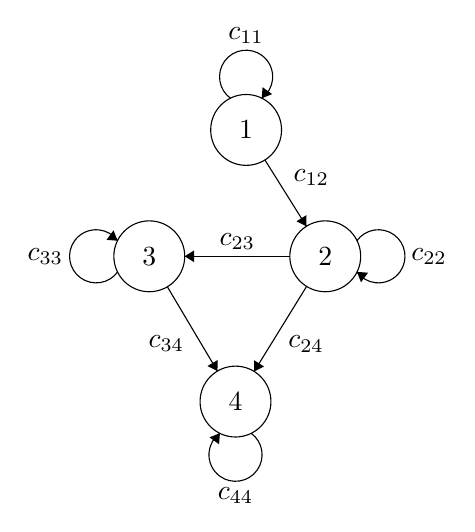
\begin{tikzpicture}[scale=0.15]
\tikzstyle{every node}+=[inner sep=0pt]
\draw [black] (41,-10.7) circle (3);
\draw (41,-10.7) node {$1$};
\draw [black] (47.7,-21.4) circle (3);
\draw (47.7,-21.4) node {$2$};
\draw [black] (32.8,-21.4) circle (3);
\draw (32.8,-21.4) node {$3$};
\draw [black] (40.1,-33.7) circle (3);
\draw (40.1,-33.7) node {$4$};
\draw [black] (42.59,-13.24) -- (46.11,-18.86);
\fill [black] (46.11,-18.86) -- (46.11,-17.91) -- (45.26,-18.44);
\draw (44.98,-14.76) node [right] {$c_{12}$};
\draw [black] (44.7,-21.4) -- (35.8,-21.4);
\fill [black] (35.8,-21.4) -- (36.6,-21.9) -- (36.6,-20.9);
\draw (40.25,-20.9) node [above] {$c_{23}$};
\draw [black] (34.33,-23.98) -- (38.57,-31.12);
\fill [black] (38.57,-31.12) -- (38.59,-30.18) -- (37.73,-30.69);
\draw (35.8,-28.8) node [left] {$c_{34}$};
\draw [black] (46.12,-23.95) -- (41.68,-31.15);
\fill [black] (41.68,-31.15) -- (42.52,-30.73) -- (41.67,-30.2);
\draw (44.53,-28.83) node [right] {$c_{24}$};
\draw [black] (41.423,-36.38) arc (54:-234:2.25);
\draw (40.1,-40.95) node [below] {$c_{44}$};
\fill [black] (38.78,-36.38) -- (37.9,-36.73) -- (38.71,-37.32);
\draw [black] (50.38,-20.077) arc (144:-144:2.25);
\draw (54.95,-21.4) node [right] {$c_{22}$};
\fill [black] (50.38,-22.72) -- (50.73,-23.6) -- (51.32,-22.79);
\draw [black] (39.677,-8.02) arc (234:-54:2.25);
\draw (41,-3.45) node [above] {$c_{11}$};
\fill [black] (42.32,-8.02) -- (43.2,-7.67) -- (42.39,-7.08);
\draw [black] (30.12,-22.723) arc (-36:-324:2.25);
\draw (25.55,-21.4) node [left] {$c_{33}$};
\fill [black] (30.12,-20.08) -- (29.77,-19.2) -- (29.18,-20.01);
\end{tikzpicture}
\end{center}
\end{minipage}
\end{example}

From the example above, we observe that we can construct a reparameterization of our model. Consider two nodes $(j,i)$. If $P_{ji}$ is not empty, then every element $p\in P_{ji}$ can be written as $p= [j=k_0\rightarrow k_1\rightarrow \hdots \rightarrow k_n=i]$
where $\{k_1, \hdots, k_{n-1}\}$ represent the intermediate nodes. For each of these paths, we define the function $d_{ji}(p)$ as the product of the weights along the path.
\begin{align*}
    d_{ji}(p):=c_{k_0,k_0}\cdot c_{k_0,k_1}\cdot\hdots\cdot c_{k_{n-2},k_{n-1}}\cdot c_{k_{n-1},k_n}=c_{k_0,k_0}\prod_{l=0}^{n-1}c_{k_l,k_{l+1}}
\end{align*}
Using this function, we compose a variable $b_{ji}$ the following way:
\begin{align*}
    b_{ji}=\begin{cases}c_{ii} & j=i\cr
    \ds\bigvee_{p\in P_{ji}}d_{ji}(p) &j\in an(i)\cr
    0 & j \in V \setminus An(i)
    \end{cases}
\end{align*}
The logic behind this creation is as follows: the coefficient between a node and itself is simply the weight associated with the node $c_{ii}$. The coefficient between two communicating nodes $j$ and $i$ is given by the path with the largest weight product. If two nodes $i$
 and $j$ do not communicate, the coefficient associated with them is 0. Using this new variable, we can rewrite equation (1) as follows:
 \begin{align*}
     X_i:= \bigvee_{j=1}^db_{ji}Z_j&& i=1,\hdots,d
 \end{align*}
 Given an ML model of $\mathbf{X}=(X_1,\hdots,X_d)$ on a DAG $\mathcal{D}$, the variables $b_{ji}$ can be formed into a $d\times d$ matrix $B$ where $B_{ji}=b_{ji}$.
 \begin{definition}When defining a max-linear model on $\mathbf{X}$, the $B$ matrix is referred to as the \textbf{max-linear coefficient matrix} and its entries are dubbed \textbf{max-linear coefficients}.
 \end{definition}For example 2.1, the B matrix would be of the form 
 \[ B=
\begin{bmatrix}
b_{11} &b_{12} & b_{13}& b_{14}\\
b_{21} &b_{22} & b_{23}& b_{24}\\
b_{31} &b_{32} & b_{33}& b_{34}\\
b_{41} &b_{42} & b_{43}& b_{44}
\end{bmatrix}=
\begin{bmatrix}
c_{11} &c_{12}c_{11} & c_{e3}c_{12}c_{11}& c_{24}c_{12}c_{11}\vee c_{34}c_{23}c_{12}c_{11}\\
0 & c_{22} & c_{23}c_{22}& c_{24}c_{22}\vee c_{34}c_{23}c_{22}\\
0&0 &c_{33} & c_{33}c_{34} \\
0& 0 & 0 & c_{44}
\end{bmatrix}
\]
To visualise the generation of the max-linear coefficient matrix from a network graph, consult section 1 of the attached code document.

\section{Introduction to Copulas}
\begin{definition}
A \textbf{Copula} is a cumulative distribution function with univariate, uniform margins\cite{nescopula}. The term is derived from Latin and refers to a bond which is apt because copulas are used to create a link between a joint distribution function and its univariate margins. This is done using Sklar's theorem \cite{incopula}.
\end{definition}

\begin{theorem}[Sklar's Theorem] Given random variables $X_1,\hdots,X_d$ with corresponding  marginal cumulative distribution functions $F_1,\hdots,F_d$, there always exists a copula $C$ such that:
\begin{align*}
    P(X_1\leq x_1, \hdots, X_d\leq x_d)=C( F_1(x_1),\hdots ,F_d(x_d)) &&\forall x_1\hdots,x_d\in\mathbb{R}
\end{align*}
This means that the joint cumulative distribution of random variables $\ds \{X_i\}_{i=1}^d $ can be represented by a function of the marginal probability distributions.
\end{theorem}

\begin{theorem}[Extension to Sklar's Theorem]
If the cumulative distribution functions (cdf) are continuous, then the copula $C$ is unique and can be retrieved by the joint cdf of the original random variable vector $(X_1,\hdots,X_d)$ after the \textbf{integral transform} has been applied to each of the components: $(F_1(X_1),\hdots,F_d(X_d))$.
\begin{proof}
In this paper, we show this result holds for the set of continuous and strictly increasing functions $\ds \{F_i\}_{i=1}^d$. The result also extends to monotonic increasing functions \cite{incopula}.
From the restriction on the functions, we know that $\forall x,y \in \mathbb{R} ,\forall i\ s.t.\ 1\leq i\leq d$ we have $x\leq y\implies F_i(x)\leq F_i(y)$. We can now use this to prove our result. 
\begin{align*}
    C( F_1(x_1),\hdots ,F_d(x_d))&=P(X_1\leq x_1,\hdots, X_d\leq x_d)\\
    &=P(F_1(X_1)\leq F_1(x_1),\hdots,F_d(X_d)\leq F_d(x_d))\\
    &=P(F_1(X_1)\leq u_1,\hdots,F_d(X_d)\leq u_d)\\
    &=P(X_1\leq F_1^{-1}(u_1),\hdots,X_d\leq F_d^{-1}(u_d))\\
    &=C(F_1(F_1^{-1}(u_1)),\hdots,F_d(F_d^{-1}(u_d)))\\
    &=C(u_1,\hdots,u_d)
\end{align*}
\end{proof}
\noindent From this we note that the copula can be set to the joint cdf of the random vector obtained by element wise integral transform.
\end{theorem}
\section{Bivariate Extreme Value Copulas}
\begin{definition}[EVC]
If a bivariate copula $C$ takes the form:
\begin{align*}
    C(u^t,v^t)=C(u,v)^t && \forall \ t>0, u,v\in[0,1] 
\end{align*}
then $C$ is termed a \textbf{bivariate extreme value copula}(BEVC) \cite{bevcbook}.

\end{definition}
\begin{definition}[Pickands representation BEVCs]
Extreme value copulas are uniquely characterized by a finite measure $\delta$ termed the \textbf{spectral measure}\cite{bevcart}. The measure $\delta$ acts on the unit simplex and defines a function $A$ referred to as the \textbf{Pickands dependence function}\cite{bevcart}.  In the bivariate case, $\delta$ or $A$ can be interchangeably used to uniquely characterize an EVC. As a result a copula $C$ is an BEVC if and only if it can be written as:
\begin{align*}
    C(u,v)=(uv)^{A\big( \frac{\log u}{\log uv} \big)} && u,v\in[0,1]\tag{2}
\end{align*}
For more background on the representation in equation (2) see McNeil \cite{bevcbook}.
\end{definition}

\subsection{Modifying the Spectral Measure}
First, we define the unit simplex: $S_2=\{(u,v)\in [0,1]^2|u+v=1 \}$. Then, the measure $\delta$ acts on $S_2$ and satisfies the condition\cite{bevcart}:
$$\int_{S_2}ud\delta(u,v)=\int_{S_2}vd\delta(u,v)=1$$
From this, it is simple to see that $\delta(S_2)=2$.
\begin{align*}
    \delta(S_2)&=\int_{S_2}d\delta(u,v)\\
    &=\int_{S_2}(u+v)d\delta(u,v)\\
    &=\int_{S_2}ud\delta(u,v)+\int_{S_2}vd\delta(u,v)=2
\end{align*}
Although the measure $\delta$ is used in many papers including Mai\cite{bevcart}, in this paper, we will consider another measure. We define $\delta^*$ such that $\ds\delta^*=\frac{\delta}{2}$. This transformation of $\delta$ is a probability measure with the unit simplex as support. In fact: 
$$(Z,Y)\thicksim \delta^* \implies \E[Z]=\E[Y]=\frac{1}{2}$$

\subsection{Pickands Dependence Function}
From the original copula measure $\delta$, the Pickands dependence function can be represented as: 
\begin{align*}
    A(t)=\int_{S_2} \max\{tu,(1-t)v\}d\delta(u,v) 
\end{align*}
When working with $\delta^*$, we use the properties of probability measures to rewrite this in terms of expectation:
$$A(t)=2*\E[(tZ\vee ((1-t)Y)]$$ 
Where $Z,Y\thicksim \delta^*$. As a consequence $A$ has the following properties\cite{bevcart}:
\begin{itemize}
    \item $A:[0,1]\rightarrow[1/2,1]$
    \item $A$ is continuous and convex
    \item $A(0)=A(1)=1$
    \item $\max \{t,1-t\}\leq A(t)\leq 1$ for $t\in[0,1]$
\end{itemize}

\subsection{Reparameterization of BEVCs}
Since we are working on the unit simplex in two dimensions, we can use a mapping from the real number line to the unit simplex to simplify our calculations. This is done using the bijection $\phi$ (defined below).
\begin{align*}
    \ds \phi: [0,1] &\rightarrow S_2\\
    \phi(x)&=(x,1-x)
\end{align*}
With this bijection, we can project the unit simplex on the real number line. This means that we can now redefine our probability measure $\delta^*$ as a univariate distribution such that:
$$\phi(X)\thicksim \delta^* \implies \E[X]=\E[1-X]=\frac{1}{2}$$
Here, $X$ has for $[0,1]$ for support. With this new random variable defined, we can wewrite our dependence function as:
$$A(t)=2* \E[(tX\vee ((1-t)(1-X))]$$

\subsection{Reparameterized Dependence Function}
Lets say our finite measure $\delta^*$ defines a random variable $\phi(X)$ with d atoms $\{q_1, \hdots, q_d\}$ each having a probability associated to it $\{p_1, \hdots, p_d\}$. Then, to calculate the copula that corresponds to $\phi(X)$, we must first calculate the dependence function:
\begin{align*}
    A(t)&=2* \E[(tX\vee (1-t)(1-X))]\\
    &=2*\sum_{i=1}^d(tq_i\vee (1-t)(1-q_i))p_i
\end{align*}
Now, we can use this to explicitly determine the form of the dependence function. Assume WLOG that the atoms are ordered such that $i<j \implies q_i<q_j \forall \ 1<i,j<d$. Then, $A(t)$ can be written as:
\begin{align*}
    A(t)=\begin{cases}
    2 (1-t)\sum_{i=1}^d(1-q_i)p_i & 0\leq t\leq 1-q_d\\
    \hdotsfor{1}\\
    2\bigg\{t\sum_{j=k}^d(q_jp_j)+(1-t)\sum_{i=1}^{k-1}(1-q_i)p_i\bigg\}& 1-q_k\leq t\leq 1-q_{k-1}\\
    \hdotsfor{1}\\
    2t\sum_{i=1}^dq_ip_i& 1-q_1\leq t\leq 1
    \end{cases}
\end{align*}
It is important to note that we have continuity at each segment. 
We can generalize this formula. The above equation assumes that we do not have any atoms at 0 or 1. Let us maintain the ordering on the set of atoms but  assume that we an atom at 0 and an atom at 1(i.e. $q_1=0$ and $q_d=1$). Then, the general form of the dependence function:
\begin{align*}
    \ds A(t)=\underbrace{2(1-t)p_1 + 2tp_d}_{K(t)}+2\sum_{i=2}^{d-1}(tq_i\vee (1-t)(1-q_i))p_i \tag{3}
\end{align*}
Where $K(t)$ is defined for readability. The piecewise description of the function now becomes:
\begin{align*}
    A(t)=\begin{cases}
    K(t)+2(1-t)\sum_{i=2}^{d-1}(1-q_i)p_i & 0\leq t\leq 1-q_{d-1}\\
    \hdotsfor{1}\\
    K(t)+2\bigg\{ t\sum_{j=k}^{d-1}(q_jp_j)+(1-t)\sum_{i=2}^{k-1}(1-q_i)p_i\bigg\}& 1-q_k\leq t\leq 1-q_{k-1}\\
    \hdotsfor{1}\\
     K(t)+2\bigg\{t\sum_{i=2}^{d-1}q_ip_i\bigg\}& 1-q_2\leq t\leq 1
    \end{cases}
\end{align*}
\subsection{Analysis of $A(t)$}
Given the piecewise dependence function $A(t)$, we may want to recover the atoms $\{q_1,\hdots,q_d\}$ and their associated probabilities $\{p_1,\hdots,p_d\}$. To do this, we use the continuity of the function at the ``kinks" $\ds \{1-q_i\}_{i=2}^{d-1}$. For any interval, $1-q_k\leq t\leq 1-q_{k-1}$, we can evaluate $A(t)$ at the endpoints and consider the difference $A(1-q_k)-A(1-q_{k-1})$.
\begin{align*}
    \underbrace{A(1-q_k)}_{(*)}&=2\bigg\{q_kp_1 + (1-q_k)p_d+ (1-q_k)\sum_{j=k}^{d-1}(q_jp_j)+q_k\sum_{i=2}^{k-1}(1-q_i)p_i\bigg\}\\
    \underbrace{A(1-q_{k-1})}_{(**)}&=2\bigg\{q_{k-1}p_1 + (1-q_{k-1})p_d+ (1-q_{k-1})\sum_{j=k}^{d-1}(q_jp_j)+q_{k-1}\sum_{i=2}^{k-1}(1-q_i)p_i\bigg\}\\
    \frac{(*)-(**)}{(q_{k-1}-q_k)}&=2\bigg\{-p_1+p_d +\sum_{j=k}^{d-1}q_jp_j -\sum_{j=2}^{k-1}p_j+\sum_{j=2}^{k-1}q_jp_j\bigg\}\\
    &=2\bigg\{ \sum_{j=1}^dq_jp_j -\sum_{j=1}^{k-1}p_j \bigg\}=2\bigg\{ \E[X]-\sum_{j=1}^{k-1}p_j\bigg\}\\
    &=2\bigg\{ \frac{1}{2}-\sum_{j=1}^{k-1}p_j \bigg\}
\end{align*}
From this, we can recover the probabilities recursively. It is worth noting that the left hand side is proportional (up to a factor of -1) to the slope of $A(t)$ on the interval $[1-q_k, 1-q _{k-1}]$ and is therefore similarly proportional to the derivative at every point in this interval.

\subsection{Representation of Bivariate EVCs}
Let us assume that we are trying to calculate the explicit form of a copula of a variable $\phi(X)$ where $X$ has the same specifications as above. The first step to using (2) to calculate the copula is to calculate $A$:
\begin{align*}
\bar{q}_i&=1-q_i \hspace{1cm} \forall 1\leq i\leq d\\
    A\big( \frac{\log u}{\log uv} \big)&=2*\sum_{i=1}^d\bigg(\frac{\log u}{\log uv}q_i\vee(1-\frac{\log u}{\log uv})\bar{q}_i\bigg)p_i\\
    &=2*\sum_{i=1}^d\bigg(\frac{\log u}{\log uv}q_i\vee\frac{\log v}{\log uv}\bar{q}_i\bigg)p_i\\
    &=2*\frac{1}{\log(uv)}\sum_{i=1}^d(q_i\log u \wedge \bar{q}_i\log v)p_i
\end{align*}
Now we use this to calculate the copula:
\begin{align*}
 C(u,v)&=(uv)^{2*\frac{1}{\log(uv)}\sum_{i=1}^d(q_i\log u \wedge \bar{q}_i\log v)p_i}\\
    &=\exp\{2*\sum_{i=1}^d(q_i\log u \wedge \bar{q}_i\log v)p_i\}\\
    &=\prod_{i=1}^d\exp\{2*q_ip_i\log u \wedge 2*\bar{q}_ip_i\log v\}\\
    &=\prod_{i=1}^d\bigg(u^{q_i}\wedge v^{\bar{q}_i}\bigg)^{2p_i} \tag{4}
\end{align*}
From this, we see that any bivariate EVC copula can be retrieved from the product of other copulas. This corroborate with Theorem 1 from \cite{bevcart}  that states that any copula $C$ can be written as 
$$C(u,v)= \prod_{i=1}^dC_{a_i,\bar{a}_i}^{p_i}$$
where $C_{a_i,\bar{a}_i}$ is a copula of the form $C_{s,t}(u,v)=\min(u^s,v^t)$ and $\sum_{i=1}^dp_i=1$. Because the spectral measure used here differs from the spectral measure by a factor of $\frac{1}{2}$ we find that the sum of our exponent is 2 rather than 1.
\pagebreak

\section{Copulas and Max Linear Models}
Let us assume that we have data that consists of  $n$ observations from $d$ sources denoted $X_1,\hdots, X_d$. If we want to use a ML model to learn more about the underlying structure and relationship between these sources, we make use of copulas. To calculate the copulas, we must calculate the following:
\begin{enumerate}
    \item The marginal cdfs $\ds\{F_1, \hdots, F_d\}$ \item The joint cdf $H(x_1,\hdots,x_d)=P(X_1\leq x_1, \hdots, X_d\leq x_d)$
    \item The copula $C(u_1,\hdots,c_d)=H(F\inv_1(u_1),\hdots,F\inv_d(u_d))$ \footnote{follows from  Theorem 2}
\end{enumerate}
\subsection{Marginal cdfs (theory)}
Assume the random variables $X_1,\hdots, X_d$ follow a ML model with i.i.d. shock random variables $Z_1,\hdots, Z_d$ and ML coefficient matrix 
\[ B=\begin{bmatrix}
&b_{11} &b_{12}&\hdots& b_{1d-1}& b_{1d}\\
&b_{21} &b_{22}&\hdots& b_{2d-1}& b_{2d}\\
&\vdots&\vdots&\ddots & \vdots& \vdots \\
&\vdots&\vdots&\hdots & \ddots& \vdots \\
&b_{d1}& b_{d2} & \hdots &b_{d-1}& b_{d}\\
\end{bmatrix}
\]
Where $b_{ij}$ is the maximum weight associated with any path from $i$ to $j$. We can calculate the marginal cdf for each of the $X_k$:
\begin{align*}
    F_{X_k}(x_k)&=P(X_k\leq x_k)=P(\bigvee_{j=1}^db_{jk}Z_j\leq x_k)=\prod_{j=1}^dP(Z_j\leq \frac{x_k}{b_{jk}})\\
    &=\prod_{j=1}^dF_{Z_j}( \frac{x_k}{b_{jk}})
\end{align*}
If we assume that $Z_i\overset{\tiny{iid}}{\thicksim}$ Fréchet $(\alpha)$ we get the following result
\begin{align*}
    F_{k}(x_k)&=\prod_{j=1}^d\exp\bigg\{{-\big(\frac{x_k}{b_{jk}}}\big)^{-\alpha}\bigg\}=\exp\bigg\{{-\sum_{j=1}^d\big(\frac{x_k}{b_{jk}}}\big)^{-\alpha}\bigg\}\\
    &=\exp\bigg\{{-x_k^{-\alpha}\sum_{j=1}^d{b_{jk}}^{\alpha}}\bigg\}\\
    \implies F_{k}\inv(u)&=\bigg(\frac{\sum_{j=1}^d{b_{jk}^\alpha}}{-\log(u)} \bigg)^{{1}/{\alpha}}
\end{align*}
It is important to note that if $j\notin An(k)$ then $b_{jk}=0$. This means that the sum $\ds \sum_{j=1}^d{b_{jk}}$ is equivalent to $\ds \sum_{j\in An(k)}{b_{jk}}$.

\subsection{Marginal cdfs (from data)}
From the data, we obserbe points of the form $$\{(X_{11},\hdots,X_{1d}), \hdots, (X_{n1}, \hdots X_{nd})\}$$
To build a copula, we need the points 
$$\{(F_1(X_{11}),\hdots,F_d(X_{1d})), \hdots, (F_1(X_{n1}), \hdots F_d(X_{nd}))\}$$
To represent a sample from $C$, because we do not have the analytic values for $\{F_1,\hdots,F_d\}$, we estimate them using the following formula:
$$\widehat{F}_i(x)=\frac{1}{n}\sum_{j=1}^n\mathbbm{1}(X_{ij}\leq x)$$
This is an application of the \textbf{rank plot} method. Essentially, for each random variable $X_{i}$, we rank all observations from smallest to greatest. Then, the rank (position in observation vector) of each observation helps us build our cdf $F_i$. The marginal cdf of each random variable evaluated at $x$ is calculated by dividing the number of observations greater than $x$ by the total number of observations. In practice, we use 
$$\widehat{F}_i(x)=\frac{1}{n+1}\sum_{j=1}^n\mathbbm{1}(X_{ij}\leq x)$$
because it leads to more tractable results\footnote{better computations when strictly bound by unit square}.

\subsection{Joint cdf}
In general, the joint cdf $H$ of random variables following a max-linear model can be calculated in the following way:
\begin{align*}
    H(x_1,\hdots, x_d)&=P(X_1\leq x_1,\hdots,X_d\leq x_d)\\
    &=P(\bigvee_{j=1}^db_{j1}Z_j\leq x_1, \hdots, \bigvee_{j=1}^db_{jd}Z_j\leq x_d)\\
    &=P(Z_1\leq{\bigwedge_{k=1}^d\frac{x_k}{b_{1k}}},\hdots, Z_d\leq\bigwedge_{k=1}^d\frac{x_k}{b_{dk}})\\
    &=\prod_{i=1}^dF_i(\bigwedge_{k=1}^d\frac{x_k}{b_{ik}})
\end{align*}
When we deal with Frechét shock, this simplifies.
\begin{align*}
    F_i(\bigwedge_{k=1}^d\frac{x_k}{b_{ik}})&=\exp\bigg\{-\bigg(\bigwedge_{k=1}^d\frac{x_k}{b_{ik}}\bigg)^{-\alpha}\bigg\}\\
    &=\exp\bigg\{-\bigvee_{k=1}^d \bigg( \frac{b_{ik}}{x_k} \bigg)^\alpha\bigg\}\\
    \implies H(x_1,\hdots, x_d)&=\prod_{i=1}^d\exp\bigg\{-\bigvee_{k=1}^d \bigg( \frac{b_{ik}}{x_k} \bigg)^\alpha\bigg\}\\
    &=\exp\bigg\{ -\sum_{i=1}^d \bigvee_{k=1}^d \bigg( \frac{b_{ik}}{x_k} \bigg)^\alpha \bigg\}\\
    &=\exp\bigg\{ -\sum_{i=1}^d \bigvee_{k=1}^d \bigg( \frac{b_{ik}}{x_k} \bigg)^\alpha \bigg\}
\end{align*}
Again we note that the index of the max operator can be changed to be in terms of ancestors. This is because for any two random variables $i,k$, if $i \notin An(k)$, then $b_{ik}=0$. So we can write 
$$H(x_1,\hdots,x_d)=\exp\bigg\{ -\sum_{k=1}^d  \bigvee_{i\in An(k)}\bigg( \frac{b_{ik}}{x_k} \bigg)^\alpha \bigg\}$$

\subsection{Building the Copula}
Now, we can put it all together to find the copula.
\begin{align*}
    C(u_1,\hdots, u_d)&=H(F_1\inv(u_1),\hdots, F_d\inv(u_d))\\
\end{align*}
When dealing with Frechét shock, the calculation becomes:
\begin{align*}
a_k&=\sum_{j=1}^d{b_{jk}^\alpha}\\
F_{k}\inv(u)&=\bigg(\frac{\sum_{j=1}^d{b_{jk}^\alpha}}{-\log(u)} \bigg)^{{1}/{\alpha}}=\bigg(\frac{a_k}{- \log(u)}\bigg)^{1/\alpha}\\
H(x_1,\hdots,x_d)&=\exp\bigg\{ -\sum_{i=1}^d \bigvee_{k=1}^d \bigg( \frac{b_{ik}}{x_k} \bigg)^\alpha \bigg\}\\
     C(u_1,\hdots, u_d)&=\exp\bigg\{ -\sum_{i=1}^d \bigvee_{k=1}^d \frac{b_{ik}^\alpha}{a_k}(-\log(u_k))\bigg\}\\
     &=\prod_{i=1}^d\exp\bigg\{- \bigvee_{k=1}^d \frac{b_{ik}^\alpha}{a_k}(-\log(u_k))\bigg\}\\
     &=\prod_{i=1}^d\exp\bigg\{- \bigvee_{k=1}^d -\log(u_k^\frac{b_{ik}^\alpha}{a_k})\bigg\}\\
     &=\prod_{i=1}^d\exp\bigg\{ \bigwedge_{k=1}^d \log(u_k^\frac{b_{ik}^\alpha}{a_k})\bigg\}\\
     \ds&=\prod_{i=1}^d \bigwedge_{k=1}^d u_k^\frac{b_{ik}^\alpha}{a_k}\tag{5}
\end{align*}
This is the copula for a ML model with Frechét shock. Note that using the same indexing trick that we have applied before, we can rewrite this as
$$C(u_1,\hdots,u_d)=\prod_{k=1}^d 1\wedge\bigg\{ \bigwedge_{i\in An(k)} u_k^\frac{b_{ik}^\alpha}{a_k}\bigg\}=\prod_{k=1}^d  \bigwedge_{i\in An(k)} u_k^\frac{b_{ik}^\alpha}{a_k}$$
ML data generated by Frechét shock can be seen in Section 2 of the coding section of this report.
\pagebreak


\section{Extreme Value Copulas and Max Linear Models}
The final purpose of this report to compare the copula that arises from the max-linear model to bivariate EVCs. For this, we will alter slightly alter the copula that arises from the ML model. We set the variables $u_1=\hdots=u_d=1$ except for two variables denoted $u_{k_1},u_{k_2}$. The goal of this is to marginalise the copula so we only consider the joint distribution of two nodes at a time. The resulting copula is then 
$$C(u_{k_1},u_{k_2})=\prod_{j=1}^du_{k_1}^{\frac{b_{jk_1}^\alpha}{a_{k_1}}}\wedge u_{k_2}^{\frac{b_{jk_2}^\alpha}{a_{k_2}}}$$
We note that $j\notin An(k_1)\cup An(k_2)$ will contribute a factor of 1 to the product. So, the copula can the the following form:
$$C(u_{k_1},u_{k_2})=\prod_{j=1,j\in An(k_1)\cup An(k_2) }^du_{k_1}^{\frac{b_{jk_1}^\alpha}{a_{k_1}}}\wedge u_{k_2}^{\frac{b_{jk_2}^\alpha}{a_{k_2}}}$$
Let $D_0=\{l:l\in An(k_1)\cap An(k_2)\}$ with $|D_0|=n$, $D_1=\{l:l\in An(k_1)\setminus An(k_2)\}$, and $D_2=\{l:l\in An(k_2)\setminus An(k_1)\}$\footnote{$|D_0|+|D_1|+|D_2|=d$}.
The above product can then be written as:
$$C(u_{k_1},u_{k_2})=\prod_{j_l\in D_1 }u_{k_1}^{\frac{b_{j_lk_1}^\alpha}{a_{k_1}}} \prod_{j_l\in D_2 }u_{k_2}^{\frac{b_{j_lk_2}^\alpha}{a_{k_2}}}\prod_{l=1,j_l\in D_0 }^n u_{k_1}^{\frac{b_{j_lk_1}^\alpha}{a_{k_1}}}\wedge u_{k_2}^{\frac{b_{j_lk_2}^\alpha}{a_{k_2}}}$$
Now, let us consider a bivariate EVC with atoms at points $\ds\{q_0,\hdots,q_{n+1}\}$ where $q_0=0$ and $q_{n+1}=1$:
$$C(u_{k_1},u_{k_2})= u_{k_1}^{2p_{n+1}} \times u_{k_2}^{2p_0}\times  \prod_{l=1}^{n} u_{k_1}^{2q_lp_l}\wedge u_{k_2}^{2(1-q_l)p_l}$$
From this, we can calculate the location of the atoms as well as their associated probabilities. First we start with the set of common ancestors $D_0$:
\begin{align*}
    \prod_{l=1,j_l\in D_0}^nu_{k_1}^{\frac{b_{j_lk_1}^\alpha}{a_{k_1}}}&\wedge u_{k_2}^{\frac{b_{j_lk_2}^\alpha}{a_{k_2}}}=\prod_{l=1}^{n} u_{k_1}^{2q_lp_l}\wedge u_{k_2}^{2(1-q_l)p_l}\\
    \implies p_l&=\frac{b_{j_lk_1}^\alpha}{2a_{k_1}}+\frac{b_{j_lk_2}^\alpha}{2a_{k_2}}\\
    \implies q_l&=\frac{\frac{b_{j_lk_1}^\alpha}{a_{k_1}}}{\frac{b_{j_lk_1}^\alpha}{a_{k_1}}+\frac{b_{j_lk_2}^\alpha}{a_{k_2}}}
\end{align*}
Second, we consider the ancestor set $D_1$:
\begin{align*}
    \prod_{j_l\in D_1 }u_{k_1}^{\frac{b_{j_lk_1}^\alpha}{a_{k_1}}} &=  u_{k_1}^{2p_{n+1}}\\
    \implies p_{n+1}&= \sum_{j_l \in D_1}\frac{b_{j_lk_1}^\alpha}{2a_{k_1}}
\end{align*}
Note that if $p_{n+1}=0$, then $An(k_1)\subseteq An(k_2)$. We have a similar result when we consider the set $D_2$:
\begin{align*}
    \prod_{j_l\in D_2 }u_{k_2}^{\frac{b_{j_lk_2}^\alpha}{a_{k_2}}} &=  u_{k_2}^{2p_{0}}\\
    \implies p_{0}&= \sum_{j_l \in D_2}\frac{b_{j_lk_2}^\alpha}{2a_{k_2}}
\end{align*}
Where we note that if $p_0=0$, then $An(k_2)\subseteq An(k_1)$.

\subsection{Calculating $A(t)$ From B}
Now, given a max linear coefficient matrix $B$, we can calculate each of the probabilities and the associated atoms. This method is explored at length in section 3 of the code section of this report.

\subsection{Calculating $C$ from $A(t)$}
Now, given the Pickands dependence function between two nodes of our ML model, we may want to generate a matrix $C$ whose entries are proportional to the entries of $B$. We define the matrix
\[ C=\begin{bmatrix}
&c_{11} &c_{12}&\hdots& c_{1d-1}& c_{1d}\\
&c_{21} &c_{22}&\hdots& c_{2d-1}& c_{2d}\\
&\vdots&\vdots&\ddots & \vdots& \vdots \\
&\vdots&\vdots&\hdots & \ddots& \vdots \\
&c_{d1}& c_{d2} & \hdots &c_{dd-1}& c_{dd}\\
\end{bmatrix}
\]
Where  $$c_{ij}=\frac{b^\alpha_{ij}}{\sum_{k=1}^db_{kj}^\alpha}$$
We assume that the Pickands dependence function between nodes $X_{i_1}$ and $X_{i_2}$ $A_{i_1i_2}(t)$ is given as the list of atoms and their probabilities. We have seen in section 4.5 that we can retrieve the probabilities from the function $A(t)$. Once we have done that, we can use the derivations from the beginning of chapter 6 to retrieve the entries of the $C$ matrix for columns $i_1$ and $i_2$. The issue arises from disorder. From function $A_{i_1i_2}(t)$, we are able to retrieve $\{c_{l1_i}, c_{li_2}| 1\leq l\leq d\}$:
\begin{align*}
    &c_{li_1}=2p_lq_l && p_l-p_lq_l=c_{li_2}
\end{align*}
However, we are unable to immediately place them into a matrix because the function $A_{i_1i_2}(t)$ will not (necessarily) give the same column order as the Pickands dependence function between two other nodes. To retrieve the form of the $C$ matrix from these, we must exploit the nature of our graphs. Since we are working on a directed acyclic graph, there will always be a ``source" node $s$ we can consider; assume WLOG $i_1=s$. We can think of the sets $D_0, D_2$ and $D_3$ as functions that act between two nodes. 
\begin{align*}
    D_0(k_1,k_2)&=\{l:l\in An(k_1)\cap An(k_2)\}\\
    D_1(k_1,k_2)&=\{l:l\in An(k_1)\setminus An(k_2)\}\\
    D_2(k_1,k_2)&=\{l:l\in An(k_2)\setminus An(k_1)\}
\end{align*}
Then, for any node $i_2$, we have the following:
\begin{align*}
    D_1(s,i_2)=D_2(s,i_2)=\varnothing
\end{align*}
Furthermore, we get 
$$D_0(s,i_2)=\begin{cases}\varnothing & s\notin An(i_2)\\
    s & s\in An(i_2)
    \end{cases}$$
Using this information, we know that, for the source node, When we compare it to another node, the only entry there is to retrieve $c_{si_2}$. This means that once we know the source node $s$, we can construct the row of matrix $C$ that corresponds to node $s$. If after doing so we remove the node $s$ from the graph, we are still left with a DAG. This means that we can apply the same logic recursively and construct $C$ row by row.  Below is the pseudo code for the recursive algorithm that computes the $C$ matrix from observed values of $A_{i_1i_2}$ works as follows:
\begin{lstlisting}
for all the node pairs (i1,i2):             #there are d*d-1 of these 
    1) calculate Pickands dependence function
    2) calculate probabilities and atoms
    3) make a list of the (c_{li1}, c_{li2}) pairs for each i1,i2
find the first node i1 where:
    all the (c_{1i1},c_{1i2}) list only has elements of the form:
        (1,0) or (1, c_{**}) for fixed c_{**} 
set this i1 to be s
fill out corresponding row in C 
recurse
\end{lstlisting}

\section{Results}
In this report, we have successfully drawn a relation between max-linear models and bivariate extreme value copulas. More specifically, we were able to retrieve the structure of a max-linear model with \f noise from data up to a normalizing constant. There is still work to be done. First, we have not investigated reading $A(t)$ from real data. Often, graphs arising from ML models have noise which make the inspection of the Pickands dependence function a lot less tractable. Secondly, the algorithm to retrieve the $C$ matrix will take a lot of time to run for large values of d.


\bibliographystyle{plain}
\bibliography{citing}
\end{document}